%-----------------------------------------------------------------------------%
\chapter{\babDua}
%-----------------------------------------------------------------------------%

Bab ini memaparkan landasan teori yang menjadi dasar penelitian.
Pembahasan dimulai dari konsep \textit{analisis sentimen} beserta tingkatan
dan pendekatannya, dilanjutkan dengan \textit{pendeteksian topik} dan berbagai
metodenya. Selanjutnya diuraikan dasar-dasar \textit{neural network}, mulai
dari arsitektur, fungsi aktivasi, \textit{backpropagation}, hingga metrik
evaluasi. Bab ini juga membahas \textit{Bidirectional Encoder Representations
from Transformers} (BERT) sebagai model representasi teks berbasis
\textit{transformer}, \textit{autoencoder} sebagai komponen kompresi
representasi, serta \textit{multi-task learning} sebagai kerangka pelatihan
model untuk beberapa tugas sekaligus.

%-------------------------------------------------------------------------%
\section{Analisis Sentimen}
%-------------------------------------------------------------------------%

Platform daring seperti media sosial, forum diskusi, dan situs ulasan
produk memungkinkan pengguna mengekspresikan pendapat secara bebas.
Hal ini menghasilkan data opini dalam jumlah besar yang terus bertambah,
sehingga muncul kebutuhan akan metode komputasional yang mampu
mengolahnya secara otomatis.

Analisis sentimen, yang juga dikenal sebagai \textit{opinion mining},
merupakan bidang dalam pemrosesan bahasa alami yang berfokus pada
identifikasi dan ekstraksi opini, sentimen, serta emosi yang terkandung
dalam teks \parencite{liu2012sentiment}. Secara umum, analisis sentimen
mengklasifikasikan opini ke dalam beberapa kategori: positif, negatif,
atau netral. Klasifikasi ini dapat dilakukan pada berbagai tingkatan,
mulai dari keseluruhan dokumen, per kalimat, hingga aspek tertentu dalam
teks. Pada penelitian ini, analisis dilakukan pada tingkat dokumen,
artinya setiap ulasan diklasifikasikan ke dalam satu label sentimen.
Pendekatan ini sesuai karena dataset yang digunakan, yakni Yelp dan IMDB,
masing-masing berisi ulasan dari satu pengguna tentang satu entitas.

Analisis sentimen umumnya dilakukan melalui dua pendekatan
\parencite{pang2002thumbs}. Pendekatan berbasis leksikon menggunakan
kamus sentimen yang berisi kata-kata beserta nilai sentimennya untuk
menentukan sentimen suatu teks. Pendekatan berbasis \textit{machine
learning} melatih model pada data ulasan berlabel sentimen, seperti
ulasan produk atau layanan, agar dapat mempelajari pola bahasa yang
berkorelasi dengan sentimen tertentu. Pendekatan ini lebih
mampu menangani variasi bahasa, konteks, dan domain yang beragam,
terutama pada data berskala besar. Penelitian ini menggunakan pendekatan
berbasis \textit{machine learning} sebagai landasan utama.

%-------------------------------------------------------------------------%
\section{Pendeteksian Topik}
%-------------------------------------------------------------------------%

Topik merujuk pada tema utama yang terkandung dalam sebuah teks.
Pendeteksian topik bertujuan menemukan tema-tema yang tersebar dalam
kumpulan dokumen tanpa label yang ditentukan sebelumnya
\parencite{blei2012probabilistic}. Setiap topik direpresentasikan
sebagai distribusi probabilitas atas sekumpulan kata, dan maknanya
dapat ditelusuri dari kata-kata yang paling sering muncul di dalamnya.
Metode ini termasuk ke dalam \textit{unsupervised learning} karena
tidak memerlukan anotasi data.

Salah satu metode pendeteksian topik yang umum digunakan adalah BERTopic
\parencite{grootendorst2022bertopic}, yang menggabungkan representasi
kontekstual dari model bahasa besar dengan \textit{clustering} untuk
menghasilkan topik yang koheren secara semantis.

Pada penelitian ini, pendeteksian topik dilakukan dengan pendekatan
\textit{clustering}. Dokumen-dokumen yang berdekatan maknanya
dikelompokkan ke dalam satu klaster, dan setiap klaster
diinterpretasikan sebagai satu topik. Pengelompokan dilakukan pada
ruang laten hasil \textit{autoencoder}, sebuah jaringan saraf yang
mengompresi teks menjadi representasi yang lebih padat namun tetap
mempertahankan informasi semantiknya.

%-------------------------------------------------------------------------%
\section{Neural Network}
%-------------------------------------------------------------------------%

Jaringan saraf tiruan (\textit{Artificial Neural Network}/ANN) adalah model
komputasi yang dirancang meniru cara kerja sistem saraf biologis manusia
\parencite{aggarwal2018neural}. Seperti neuron biologis yang saling
terhubung melalui sinapsis, ANN terdiri dari unit-unit komputasi yang
saling terhubung melalui bobot yang dapat disesuaikan. Proses pembelajaran
berlangsung melalui penyesuaian bobot-bobot tersebut berdasarkan data
pelatihan.

Secara umum, arsitektur ANN tersusun atas tiga komponen utama
\parencite{dasilva2017}. Pertama, \textit{input layer}, yaitu lapisan yang
menerima data mentah dari luar sistem dan meneruskannya ke lapisan berikutnya
tanpa melakukan transformasi. Kedua, \textit{hidden layer}, yaitu lapisan
yang menerapkan fungsi aktivasi untuk mengidentifikasi pola kompleks dari
data. Ketiga, \textit{output layer}, yaitu lapisan yang menghasilkan prediksi
akhir berdasarkan representasi yang telah dibangun oleh lapisan-lapisan
sebelumnya.

Gambar~\ref{fig:biological_nn} dan Gambar~\ref{fig:artificial_nn}
menunjukkan perbandingan antara jaringan saraf biologis dan ANN.

\begin{figure}[H]
    \centering
    \begin{minipage}{0.48\textwidth}
        \centering
        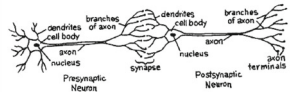
\includegraphics[width=\textwidth]{assets/pics/Aggarwal/Dendrit (Biological Neural Nework).png}
        \caption{Ilustrasi \textit{neural network} secara biologis
        \parencite{aggarwal2018neural}}
        \label{fig:biological_nn}
    \end{minipage}
    \hfill
    \begin{minipage}{0.48\textwidth}
        \centering
        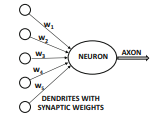
\includegraphics[width=\textwidth]{assets/pics/Aggarwal/NN ML.png}
        \caption{\textit{Artificial Neural Network} dengan representasi
        bobot sinapsis \parencite{aggarwal2018neural}}
        \label{fig:artificial_nn}
    \end{minipage}
\end{figure}

Dalam bentuk paling sederhananya, sebuah \textit{neural network} hanya
memiliki satu lapisan komputasi yang disebut \textit{perceptron}. Pada
arsitektur ini, terdapat $n$ neuron \textit{input} yang meneruskan fitur ke
satu neuron \textit{output} melalui sekumpulan bobot. Nilai \textit{output}
diperoleh dari penjumlahan bobot yang dikalikan dengan masing-masing nilai
\textit{input}, ditambah sebuah nilai \textit{bias} $b$ yang berfungsi
menggeser ambang batas keputusan model. Secara matematis, prediksi
\textit{output} dirumuskan sebagai:

\begin{equation}
    z = \mathbf{w} \cdot \mathbf{x} + b = \sum_{i=1}^{n} w_i x_i + b.
    \label{eq:perceptron}
\end{equation}

\noindent dengan $\mathbf{w}$ adalah vektor bobot, $\mathbf{x}$ adalah vektor
input, dan $b$ adalah skalar bias.

\textit{Perceptron} hanya mampu memodelkan hubungan linier antara
\textit{input} dan \textit{output}, sehingga tidak dapat menangani pola
yang lebih kompleks. Untuk mengatasi keterbatasan ini, digunakan
\textit{multilayer neural network} yang memiliki satu atau lebih
\textit{hidden layer} di antara \textit{input layer} dan \textit{output
layer}. Setiap lapisan menerima input dari lapisan sebelumnya dan
meneruskannya searah menuju \textit{output layer}. Pola aliran satu arah
seperti ini dikenal sebagai \textit{feed-forward}, dan arsitekturnya
ditunjukkan pada Gambar~\ref{fig:feedforward}.

\begin{figure}[H]
    \centering
    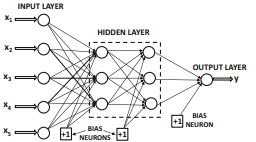
\includegraphics[width=0.7\textwidth]{assets/pics/Aggarwal/Multi Layer Bias.png}
    \caption{Arsitektur \textit{feed-forward neural network}
    \parencite{aggarwal2018neural}}
    \label{fig:feedforward}
\end{figure}

Misalkan terdapat $k$ \textit{hidden layer} dengan masing-masing $p_1,
\ldots, p_k$ neuron, $\mathbf{x}$ sebagai vektor input berisi $n$ neuron,
$\mathbf{h}_1, \ldots, \mathbf{h}_k$ sebagai keluaran tiap \textit{hidden
layer} setelah melewati fungsi aktivasi, dan $\mathbf{o}$ sebagai vektor
output berisi $m$ neuron. Matriks bobot $\mathbf{W}_1$ berdimensi
$n \times p_1$ menghubungkan \textit{input layer} dengan \textit{hidden
layer} pertama, $\mathbf{W}_r$ berdimensi $p_{r-1} \times p_r$
menghubungkan antar \textit{hidden layer}, dan $\mathbf{W}_{k+1}$
berdimensi $p_k \times m$ menghubungkan \textit{hidden layer} terakhir ke
\textit{output layer}. Proses komputasi pada tiap lapisan dirumuskan
sebagai:

\vspace{-1em}
\setlength{\abovedisplayskip}{0pt}
\begin{align}
    \mathbf{h}_1     &= \phi_1(\mathbf{W}_1^\top \mathbf{x}),
        \label{eq:input_to_hidden} \\
    \mathbf{h}_{r+1} &= \phi_{r+1}(\mathbf{W}_{r+1}^\top \mathbf{h}_r),
        \quad r \in \{1, \ldots, k-1\}, \label{eq:hidden_to_hidden} \\
    \mathbf{o}       &= \phi_0(\mathbf{W}_{k+1}^\top \mathbf{h}_k).
        \label{eq:hidden_to_output}
\end{align}

\noindent dengan $\phi_i$ adalah fungsi aktivasi yang diterapkan pada lapisan
ke-$i$. Output akhir $\mathbf{o}$ merupakan hasil transformasi bertingkat
dari input $\mathbf{x}$ melalui seluruh lapisan jaringan secara berurutan.

%-------------------------------------------------------------------------%
\subsection{Fungsi Aktivasi}
%-------------------------------------------------------------------------%

Fungsi aktivasi digunakan dalam \textit{neural network} untuk memberikan
sifat nonlinier pada model. Tanpa fungsi aktivasi, output jaringan hanya
merupakan transformasi linier dari input sehingga tidak mampu menangkap
pola yang kompleks \parencite{goodfellow2016}. Pada penelitian ini, digunakan tiga fungsi aktivasi utama,
yaitu \textit{softmax}, ReLU, dan GELU, yang masing-masing dijelaskan
berikut.

%-------------------------------------------------------------------------%
\subsubsection{\textit{Softmax}}
%-------------------------------------------------------------------------%

Fungsi \textit{softmax} digunakan untuk mengubah vektor bernilai real menjadi 
distribusi probabilitas pada $K$ kelas. Melalui proses ini, setiap nilai keluaran 
berada pada rentang 0 hingga 1, dengan total seluruh probabilitas sama dengan 1. 
Untuk vektor masukan $\mathbf{v} = (v_1, v_2, \ldots, v_K)$, fungsi \textit{softmax}
pada elemen ke-$j$ didefinisikan sebagai:

\vspace{-1em}
\setlength{\abovedisplayskip}{0pt}
\begin{equation}
    \phi(\mathbf{v})_j = \frac{e^{v_j}}{\displaystyle\sum_{k=1}^{K} e^{v_k}}.
    \label{eq:softmax}
\end{equation}

\noindent dengan $e$ adalah bilangan Euler bernilai sekitar $2{,}718$. Elemen dengan nilai $v_j$ 
yang lebih besar menghasilkan $e^{v_j}$ yang
lebih besar, sehingga probabilitas $\phi(\mathbf{v})_j$ yang diperoleh
juga lebih tinggi. Fungsi \textit{softmax} umum digunakan pada
lapisan keluaran jaringan untuk tugas klasifikasi multikelas karena
keluarannya dapat langsung diinterpretasikan sebagai probabilitas prediksi
tiap kelas.

%-------------------------------------------------------------------------%
\subsubsection{\textit{Rectified Linear Unit} (ReLU)}
%-------------------------------------------------------------------------%

\textit{Rectified Linear Unit} (ReLU) mengatasi masalah \textit{vanishing
gradient} dengan cara meneruskan nilai \textit{input} apa adanya jika
positif, dan mengembalikan nol jika negatif:

\vspace{-1em}
\setlength{\abovedisplayskip}{0pt}
\begin{equation}
    \phi(v) = \max\{v,\, 0\}.
    \label{eq:relu}
\end{equation}

ReLU lebih efisien secara komputasi dan lebih mudah dilatih pada jaringan
yang dalam, karena gradiennya selalu bernilai 1 untuk \textit{input}
positif sehingga informasi pembaruan tidak melemah saat merambat mundur
melalui banyak lapisan.

%-------------------------------------------------------------------------%
\subsubsection{\textit{Gaussian Error Linear Unit} (GELU)}
%-------------------------------------------------------------------------%

\textit{Gaussian Error Linear Unit} (GELU) digunakan sebagai 
fungsi aktivasi pada arsitektur \textit{Transformer} seperti BERT \parencite{hendrycks2016}. Berbeda dengan ReLU 
yang mengubah seluruh nilai negatif menjadi nol, GELU mengatur kontribusi 
setiap nilai \textit{input} berdasarkan probabilitas kumulatif distribusi 
Gaussian pada nilai tersebut:

\vspace{-1em}
\setlength{\abovedisplayskip}{0pt}
\begin{equation}
    \phi(v) = v \cdot \Phi(v) = v \cdot \frac{1}{2}\left[1 +
    \operatorname{erf}\!\left(\frac{v}{\sqrt{2}}\right)\right].
    \label{eq:gelu}
\end{equation}

\noindent dengan $\Phi(v)$ adalah fungsi distribusi kumulatif Gaussian standar,
dan $\operatorname{erf}(\cdot)$ adalah fungsi error dengan rentang nilai
$[-1, 1]$, sehingga $\Phi(v) \in [0, 1]$. Untuk $v$ besar dan positif,
GELU mendekati perilaku ReLU, sedangkan di sekitar nol transisinya
berlangsung mulus.

\begin{figure}[H]
    \centering
    \resizebox{\textwidth}{!}{%
        \begin{tabular}{ccc}
            \actplot{Softmax (2 kelas)}{%
                \addplot[teal, ultra thick] {exp(x)/(exp(x)+exp(-x))};
                \addplot[dashed, gray!60] coordinates {(-4.2,1)(4.2,1)};
            }{-0.2}{1.3}
            &
            \actplot{ReLU}{%
                \addplot[red!75!black, ultra thick] {max(x,0)};
            }{-0.8}{4.5}
            &
            \actplot{GELU}{%
                \addplot[blue!70!black, ultra thick]
                    {x * (1 + tanh(sqrt(2/pi) * (x + 0.044715 * x^3))) / 2};
            }{-0.8}{4.5}
        \end{tabular}%
    }
    \caption{Grafik fungsi aktivasi: \textit{Softmax}, ReLU, dan GELU}
    \label{fig:activation_functions}
\end{figure}

Perbandingan ketiga fungsi aktivasi ditunjukkan pada
Gambar~\ref{fig:activation_functions}.

%-------------------------------------------------------------------------%
\subsection{Fungsi \textit{Loss}}
%-------------------------------------------------------------------------%

Fungsi \textit{loss} mengukur seberapa jauh prediksi model menyimpang dari
nilai yang sebenarnya. Untuk tugas klasifikasi multikelas,
\textit{categorical cross-entropy loss} merupakan pilihan yang umum
digunakan \parencite{aggarwal2018neural}:

\begin{equation}
    L = -\sum_{i=1}^{n} \sum_{j=1}^{k} y_{ij} \log(\hat{y}_{ij}).
    \label{eq:categorical_crossentropy}
\end{equation}

\noindent dengan $n$ adalah jumlah sampel, $k$ adalah jumlah kelas, $y_{ij}$
adalah label aktual dalam bentuk \textit{one-hot encoded} bernilai 1
jika sampel ke-$i$ termasuk kelas ke-$j$ dan 0 jika tidak, serta
$\hat{y}_{ij}$ adalah probabilitas prediksi model untuk sampel ke-$i$
pada kelas ke-$j$.

%-------------------------------------------------------------------------%
\subsection{\textit{Backpropagation}}
%-------------------------------------------------------------------------%

Setelah nilai \textit{loss} diperoleh, langkah berikutnya dalam proses
pelatihan adalah menghitung gradien terhadap parameter model untuk
menentukan arah pembaruan bobot. Proses tersebut dilakukan menggunakan
algoritma \textit{backpropagation}
\parencite{aggarwal2018neural}.

\textit{Backpropagation} bekerja dengan merambatkan informasi kesalahan
dari lapisan keluaran menuju lapisan sebelumnya untuk menghitung seberapa
besar kontribusi masing-masing parameter terhadap nilai
\textit{loss}. Perhitungan tersebut dilakukan menggunakan aturan rantai
(\textit{chain rule}), karena keluaran model umumnya diperoleh melalui
serangkaian fungsi yang saling bergantung.

Hubungan tersebut dapat dijelaskan menggunakan graf komputasi pada
Gambar~\ref{fig:backprop_structure}.

\begin{figure}[H]
\centering
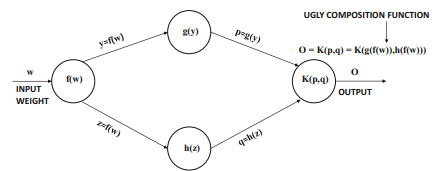
\includegraphics[width=0.6\textwidth]
{assets/pics/Aggarwal/NN Backprop.png}
\caption{Ilustrasi graf komputasi pada proses
\textit{backpropagation}
\parencite{aggarwal2018neural}}
\label{fig:backprop_structure}
\end{figure}

Pada Gambar~\ref{fig:backprop_structure}, parameter $w$ diproses melalui
beberapa tahapan transformasi hingga menghasilkan keluaran akhir $o$.
Keluaran tersebut diperoleh dari dua jalur komputasi yang digabungkan
melalui fungsi:

\begin{equation}
o
=
K(g(f(w)),h(f(w)))
\label{eq:output_composite}
\end{equation}

Persamaan~\ref{eq:output_composite} menunjukkan bahwa keluaran merupakan
fungsi komposit terhadap parameter $w$. Oleh karena itu, pengaruh perubahan
parameter terhadap nilai \textit{loss} dihitung menggunakan aturan rantai
sebagai berikut:

\begin{equation}
\frac{\partial L}{\partial w}
=
\frac{\partial L}{\partial o}
\left(
\frac{\partial o}{\partial p}
\cdot
\frac{\partial p}{\partial y}
\cdot
\frac{\partial y}{\partial w}
+
\frac{\partial o}{\partial q}
\cdot
\frac{\partial q}{\partial z}
\cdot
\frac{\partial z}{\partial w}
\right)
\label{eq:backprop_chain_rule}
\end{equation}

Pada Persamaan~\ref{eq:backprop_chain_rule},
$\partial L/\partial o$ menyatakan perubahan nilai
\textit{loss} terhadap perubahan keluaran model, sedangkan suku di dalam
tanda kurung menyatakan pengaruh parameter terhadap keluaran melalui
masing-masing jalur komputasi. Gradien diperoleh dengan mengalikan turunan
lokal pada setiap tahapan transformasi dan menjumlahkan kontribusi dari
seluruh jalur yang memengaruhi keluaran.

Proses penyebaran gradien dari keluaran menuju parameter pada tahapan
komputasi sebelumnya inilah yang disebut sebagai
\textit{backpropagation}.


%-------------------------------------------------------------------------%
\subsection{Teknik Optimasi}
%-------------------------------------------------------------------------%

Proses optimasi merupakan tahapan pencarian parameter yang menghasilkan
nilai fungsi \textit{loss} sekecil mungkin selama pelatihan
\parencite{zhang2023}. Gradien yang diperoleh dari \textit{backpropagation}
digunakan untuk memperbarui bobot model secara iteratif.

%-------------------------------------------------------------------------%
\subsubsection{\textit{Stochastic Gradient Descent} (SGD)}
%-------------------------------------------------------------------------%

\textit{Stochastic Gradient Descent} (SGD) adalah algoritma optimasi yang
diperkenalkan oleh \parencite{rumelhart1986} untuk meminimalkan fungsi
\textit{loss} $L(\mathbf{w})$ secara iteratif dengan memperbarui bobot
ke arah negatif gradiennya:

\vspace{-1em}
\setlength{\abovedisplayskip}{0pt}
\begin{equation}
    \mathbf{w}^{[t+1]} = \mathbf{w}^{[t]} - \eta \nabla L(\mathbf{w})^{[t]}.
    \label{eq:sgd}
\end{equation}

\noindent dengan $\mathbf{w}^{[t]}$ adalah vektor bobot pada iterasi ke-$t$,
$\nabla L(\mathbf{w})^{[t]}$ adalah vektor gradien fungsi \textit{loss}
terhadap bobot pada iterasi ke-$t$, dan $\eta$ adalah skalar
\textit{learning rate} yang mengontrol besar langkah pembaruan. Nilai
$\eta$ yang terlalu kecil memperlambat konvergensi, sedangkan nilai yang
terlalu besar dapat membuat pelatihan tidak stabil.

%-------------------------------------------------------------------------%
\subsubsection{\textit{Adaptive Moment Estimation} (Adam)}
%-------------------------------------------------------------------------%

\textit{Adaptive Moment Estimation} (Adam), yang dikemukakan oleh
\parencite{kingma2017}, mengembangkan SGD dengan mengadaptasi
\textit{learning rate} secara individual untuk setiap parameter. Adaptasi
ini didasarkan pada dua estimasi momen gradien: momen pertama
$\mathbf{v}^{[t]}$ terhadap gradien itu sendiri, dan momen kedua
$\mathbf{s}^{[t]}$ terhadap kuadrat gradien:

\vspace{-1em}
\setlength{\abovedisplayskip}{0pt}
\begin{equation}
    \mathbf{v}^{[t]} = \beta_1 \mathbf{v}^{[t-1]}
    + (1 - \beta_1) \nabla L(\mathbf{w})^{[t]}.
    \label{eq:adam_first_moment}
\end{equation}
\begin{equation}
    \mathbf{s}^{[t]} = \beta_2 \mathbf{s}^{[t-1]}
    + (1 - \beta_2) \left(\nabla L(\mathbf{w})^{[t]}\right)^2.
    \label{eq:adam_second_moment}
\end{equation}

\noindent dengan $\beta_1$ dan $\beta_2$ adalah skalar koefisien peluruhan yang
mengontrol pengaruh gradien lama terhadap estimasi saat ini. Karena kedua
momen diinisialisasi dengan nol, estimasinya cenderung bias ke nol pada
iterasi awal. Koreksi bias dilakukan dengan normalisasi:

\vspace{-1em}
\setlength{\abovedisplayskip}{0pt}
\begin{equation}
    \hat{\mathbf{v}}^{[t]} = \frac{\mathbf{v}^{[t]}}{1 - \beta_1^t},
    \qquad
    \hat{\mathbf{s}}^{[t]} = \frac{\mathbf{s}^{[t]}}{1 - \beta_2^t}.
    \label{eq:adam_bias_correction}
\end{equation}

Seiring bertambahnya $t$, nilai $\beta_1^t$ dan $\beta_2^t$ mendekati nol
sehingga koreksi ini semakin tidak berpengaruh. Pembaruan bobot dilakukan
menggunakan kedua momen yang telah dikoreksi:

\vspace{-1em}
\setlength{\abovedisplayskip}{0pt}
\begin{equation}
    \mathbf{w}^{[t+1]} = \mathbf{w}^{[t]}
    - \frac{\eta}{\sqrt{\hat{\mathbf{s}}^{[t]}} + \epsilon}\,
    \hat{\mathbf{v}}^{[t]}.
    \label{eq:adam_update}
\end{equation}

\noindent dengan $\epsilon = 10^{-8}$ adalah skalar untuk mencegah pembagian
dengan nol \parencite{zhang2023}. Pembagian dengan
$\sqrt{\hat{\mathbf{s}}^{[t]}}$ memperkecil langkah pembaruan untuk
parameter dengan gradien besar dan berfluktuasi, serta memperbesar untuk
parameter dengan gradien kecil dan konsisten.

%-------------------------------------------------------------------------%
\subsection{Regularisasi}
%-------------------------------------------------------------------------%

Dalam melatih model, terdapat dua kondisi yang perlu dihindari, yaitu
\textit{underfitting} dan \textit{overfitting}.
\textit{Underfitting} terjadi ketika model gagal mempelajari pola data
pelatihan, ditandai dengan bias yang tinggi. \textit{Overfitting} terjadi
ketika model terlalu menghafalkan data pelatihan sehingga performanya
menurun pada data baru, ditandai dengan variansi yang tinggi
\parencite{goodfellow2016}.

Gambar~\ref{fig:underfitting_overfitting} menunjukkan hubungan antara
kompleksitas model dengan bias, variansi, dan total error. Bias menurun
seiring meningkatnya kompleksitas model, sementara variansi justru
meningkat. Total error yang merupakan kombinasi keduanya mencapai nilai
minimum pada titik kompleksitas optimal.

\begin{figure}[H]
    \centering
    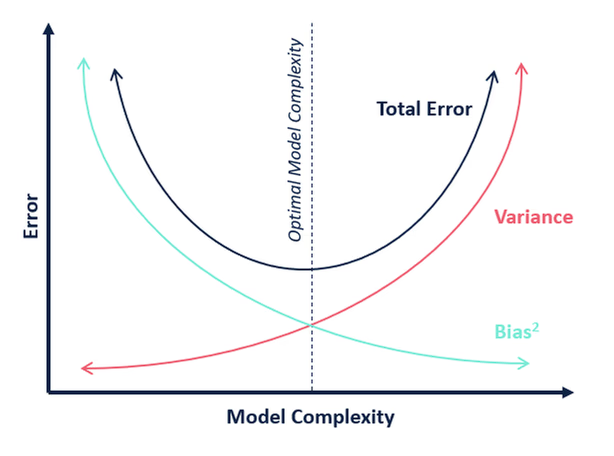
\includegraphics[width=0.6\textwidth]{assets/pics/Aggarwal/NN Regularization.png}
    \caption{Ilustrasi \textit{bias-variance tradeoff} terhadap kompleksitas
    model (\cite{aggarwal2018neural}, telah diolah kembali)}
    \label{fig:underfitting_overfitting}
\end{figure}

Untuk mencegah \textit{overfitting}, salah satu teknik yang digunakan
adalah \textit{weight decay} atau $L_2$ \textit{regularization}, yang
menambahkan penalti pada fungsi \textit{loss} proporsional terhadap besar
bobot model:

\begin{equation}
    \tilde{L}(\mathbf{w}) = L(\mathbf{w}) + \frac{\lambda}{2}
    \|\mathbf{w}\|^2.
    \label{eq:l2_regularization}
\end{equation}

\noindent dengan $L(\mathbf{w})$ adalah fungsi \textit{loss} asal,
$\|\mathbf{w}\|^2$ adalah jumlah kuadrat seluruh bobot dalam model, dan
$\lambda$ adalah skalar yang mengontrol kekuatan penalti.

Teknik lain yang digunakan adalah \textit{dropout}, yang menonaktifkan
neuron secara acak selama pelatihan agar jaringan tidak terlalu
bergantung pada neuron tertentu \parencite{srivastava2014dropout}. Untuk
vektor aktivasi $\mathbf{h} \in \mathbb{R}^p$, setiap neuron ke-$i$
dikalikan dengan variabel acak Bernoulli:

\begin{equation}
    m_i \sim \text{Bernoulli}(1 - p_{\text{drop}}), \qquad
    \tilde{h}_i = \frac{m_i}{1 - p_{\text{drop}}} \cdot h_i.
    \label{eq:dropout}
\end{equation}

\noindent dengan $p_{\text{drop}} \in [0,1]$ adalah probabilitas neuron
dinonaktifkan, dan faktor $1/(1-p_{\text{drop}})$ menyeimbangkan skala
aktivasi akibat neuron yang dinonaktifkan. Pada tahap evaluasi,
\textit{dropout} tidak diterapkan dan seluruh neuron digunakan
sepenuhnya ($\tilde{\mathbf{h}} = \mathbf{h}$).

Teknik lain yang juga memberikan efek regularisasi adalah \textit{Batch
Normalization} (BatchNorm), yang menormalisasi aktivasi berdasarkan
statistik \textit{mini-batch} untuk mempercepat dan menstabilkan
pelatihan \parencite{ioffe2015batch}. Untuk aktivasi
$\mathcal{B} = \{h_1, \ldots, h_m\}$ pada satu \textit{mini-batch}:

\begin{equation}
    \hat{h}_i = \frac{h_i - \mu_{\mathcal{B}}}
    {\sqrt{\sigma_{\mathcal{B}}^2 + \epsilon}}, \qquad
    \text{BN}(h_i) = \gamma \hat{h}_i + \beta.
    \label{eq:batchnorm}
\end{equation}

\noindent dengan $\mu_{\mathcal{B}}$ dan $\sigma_{\mathcal{B}}^2$
masing-masing adalah rata-rata dan variansi \textit{batch}, $\epsilon$
adalah skalar kecil pencegah pembagian dengan nol, serta $\gamma$ dan
$\beta$ adalah parameter skala dan pergeseran yang dipelajari agar
kapasitas representasi jaringan tetap terjaga. Pada tahap evaluasi,
$\mu_{\mathcal{B}}$ dan $\sigma_{\mathcal{B}}^2$ digantikan dengan
estimasi rata-rata bergerak yang dikumpulkan selama pelatihan.

%-------------------------------------------------------------------------%
\subsection{Metrik Evaluasi}
%-------------------------------------------------------------------------%

Tahap evaluasi bertujuan untuk mengukur kinerja model pada tugas
klasifikasi sentimen maupun klasterisasi topik. Evaluasi klasifikasi
dilakukan menggunakan metrik yang diturunkan dari
\textit{confusion matrix}, sedangkan evaluasi hasil klasterisasi topik
dilakukan menggunakan metrik \textit{topic coherence} dan
\textit{topic diversity}. Masing-masing metrik dijelaskan pada
subsubbab berikut.

%-------------------------------------------------------------------------%
\subsubsection{Metrik Evaluasi Klasifikasi}
%-------------------------------------------------------------------------%

Setelah model dilatih, performa klasifikasi dievaluasi menggunakan data
yang tidak digunakan selama proses pelatihan. Evaluasi didasarkan pada
\textit{confusion matrix}, yaitu tabel yang membandingkan hasil prediksi
model dengan label aktual. Dari tabel tersebut diperoleh empat komponen
dasar, yaitu \textit{True Positive} (TP), \textit{True Negative} (TN),
\textit{False Positive} (FP), dan \textit{False Negative} (FN). TP
menunjukkan jumlah sampel positif yang diprediksi dengan benar, TN
menunjukkan jumlah sampel negatif yang diprediksi dengan benar, FP
menunjukkan jumlah sampel negatif yang salah diprediksi sebagai positif,
sedangkan FN menunjukkan jumlah sampel positif yang salah diprediksi
sebagai negatif.

Berdasarkan keempat komponen tersebut, digunakan empat metrik evaluasi
utama, yaitu akurasi, \textit{precision}, \textit{recall}, dan
F1-\textit{Score}.

Akurasi mengukur proporsi keseluruhan prediksi yang benar terhadap seluruh
sampel pengujian.

\begin{equation}
    \text{Accuracy} =
    \frac{TP + TN}{TP + TN + FP + FN}
    \label{eq:accuracy}
\end{equation}

\textit{Precision} mengukur ketepatan model ketika memprediksi suatu
sampel sebagai kelas positif, yaitu proporsi prediksi positif yang benar.

\begin{equation}
    \text{Precision} =
    \frac{TP}{TP + FP}
    \label{eq:precision}
\end{equation}

\textit{Recall} mengukur kemampuan model dalam menemukan seluruh sampel
positif yang sebenarnya.

\begin{equation}
    \text{Recall} =
    \frac{TP}{TP + FN}
    \label{eq:recall}
\end{equation}

Karena \textit{precision} dan \textit{recall} sering kali saling
berkompromi, keduanya dikombinasikan menggunakan F1-\textit{Score},
yaitu rata-rata harmonik antara kedua metrik tersebut.

\begin{equation}
    \text{F1-Score}
    =
    2
    \times
    \frac{\text{Precision} \times \text{Recall}}
    {\text{Precision} + \text{Recall}}
    =
    \frac{2TP}{2TP + FP + FN}
    \label{eq:f1score}
\end{equation}

F1-\textit{Score} memberikan ukuran yang lebih seimbang dibandingkan
akurasi, terutama pada dataset yang memiliki distribusi kelas tidak
seimbang.

%-------------------------------------------------------------------------%
\subsubsection{Metrik Evaluasi Topik}
\label{sec:topic_eval}
%-------------------------------------------------------------------------%

Kualitas hasil klasterisasi topik dapat dievaluasi menggunakan berbagai
metrik kuantitatif. Pada penelitian ini digunakan dua metrik, yaitu
\textit{topic coherence} dan \textit{topic diversity}. Kedua metrik
dihitung langsung dari dokumen hasil klasterisasi tanpa memerlukan model
eksternal.

\textit{Topic coherence} mengukur sejauh mana kata-kata teratas dalam
suatu topik memiliki keterkaitan semantik melalui kemunculan bersama
(\textit{co-occurrence}) pada dokumen yang sama. Penelitian ini
menggunakan metrik \textit{Normalized Pointwise Mutual Information}
(NPMI). Misalkan $\mathcal{D}_k$ adalah himpunan dokumen pada klaster
ke-$k$ dan $\{w_1,w_2,\ldots,w_N\}$ merupakan $N$ kata teratas pada
klaster tersebut setelah proses penghapusan \textit{stop words}.
Probabilitas kemunculan setiap kata dan probabilitas kemunculan
bersamanya didefinisikan sebagai

\begin{align}
    p(w_i)
    &= \frac{|\{d \in \mathcal{D}_k : w_i \in d\}|}
    {|\mathcal{D}_k|},\\[4pt]
    p(w_j)
    &= \frac{|\{d \in \mathcal{D}_k : w_j \in d\}|}
    {|\mathcal{D}_k|},\\[4pt]
    p(w_i,w_j)
    &= \frac{|\{d \in \mathcal{D}_k :
    w_i \in d \text{ dan } w_j \in d\}|}
    {|\mathcal{D}_k|}.
\end{align}

Nilai \textit{Pointwise Mutual Information} (PMI) dihitung sebagai

\begin{equation}
    \mathrm{PMI}(w_i,w_j)
    =
    \log
    \frac{p(w_i,w_j)+\varepsilon}
    {p(w_i)p(w_j)+\varepsilon}
    \label{eq:pmi}
\end{equation}

dengan $\varepsilon = 10^{-10}$ digunakan untuk menghindari pembagian
dengan nol. Selanjutnya nilai PMI dinormalisasi menjadi NPMI.

\begin{equation}
    \mathrm{NPMI}(w_i,w_j)
    =
    \frac{\mathrm{PMI}(w_i,w_j)}
    {-\log(p(w_i,w_j)+\varepsilon)}
    \label{eq:npmi}
\end{equation}

Nilai NPMI berada pada rentang $[-1,1]$, di mana nilai yang semakin
mendekati $1$ menunjukkan bahwa kedua kata semakin sering muncul
bersama. Skor \textit{topic coherence} untuk setiap klaster dihitung
sebagai rata-rata nilai NPMI seluruh pasangan kata.

\begin{equation}
    \mathrm{TC}_k
    =
    \frac{1}{\binom{N}{2}}
    \sum_{j=2}^{N}
    \sum_{i=1}^{j-1}
    \mathrm{NPMI}(w_i,w_j)
    \label{eq:tc_cluster}
\end{equation}

Nilai koherensi keseluruhan diperoleh melalui rata-rata seluruh klaster.

\begin{equation}
    \overline{\mathrm{TC}}
    =
    \frac{1}{K}
    \sum_{k=1}^{K}
    \mathrm{TC}_k
    \label{eq:tc_mean}
\end{equation}

Apabila suatu klaster memiliki kurang dari dua kata unik, maka nilai
koherensinya ditetapkan sebesar $0$.

\textit{Topic diversity} mengukur tingkat keberagaman kosakata antar
topik. Semakin sedikit kata yang muncul berulang pada topik berbeda,
semakin tinggi nilai \textit{topic diversity}. Misalkan $\mathcal{W}_k$
adalah himpunan $N$ kata teratas pada klaster ke-$k$, sedangkan himpunan
seluruh kata unik didefinisikan sebagai

\[
\mathcal{U}
=
\bigcup_{k=1}^{K}\mathcal{W}_k.
\]

Nilai \textit{topic diversity} dihitung menggunakan

\begin{equation}
    \mathrm{TD}
    =
    \frac{|\mathcal{U}|}
    {\displaystyle\sum_{k=1}^{K}|\mathcal{W}_k|}
    \label{eq:td}
\end{equation}

Nilai $\mathrm{TD}=1$ menunjukkan bahwa seluruh kata teratas dari setiap
topik berbeda satu sama lain, sedangkan nilai yang semakin kecil
menunjukkan semakin banyak kosakata yang tumpang tindih antar topik.

%-------------------------------------------------------------------------%
\section{\textit{Autoencoder}}
%-------------------------------------------------------------------------%

Pemahaman tentang arsitektur \textit{feed-forward neural network} menjadi
landasan untuk memahami \textit{autoencoder}, yang pada dasarnya adalah
sebuah jaringan saraf yang dilatih untuk merekonstruksi inputnya
\parencite{goodfellow2016}. Karena tidak memerlukan label,
\textit{autoencoder} termasuk ke dalam kategori \textit{unsupervised
learning} \parencite{hinton2006reducing}.

Arsitektur \textit{autoencoder} \parencite{vincent2010stacked} terdiri
dari dua komponen utama: \textit{encoder} yang memetakan representasi
input dari dimensi tinggi ke dimensi yang lebih rendah, dan
\textit{decoder} yang merekonstruksi representasi tersebut ke dimensi
semula. Lapisan tersempit di antara keduanya disebut \textit{bottleneck}
atau ruang laten. Arsitektur lengkapnya ditunjukkan pada
Gambar~\ref{fig:autoencoder_architecture}.

\begin{figure}[H]
    \centering
    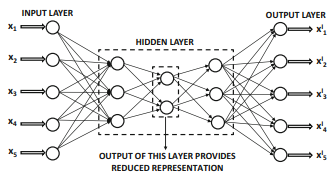
\includegraphics[width=0.75\textwidth]{assets/pics/Aggarwal/Autoencoder.png}
    \caption{Arsitektur \textit{autoencoder} menunjukkan proses
    \textit{encoding} dan \textit{decoding} \parencite{aggarwal2018neural}}
    \label{fig:autoencoder_architecture}
\end{figure}

%-------------------------------------------------------------------------%
\subsection{\textit{Encoder} dan \textit{Decoder}}
%-------------------------------------------------------------------------%

Secara formal, misalkan $\mathbf{x} \in \mathbb{R}^D$ adalah vektor input
berdimensi $D$. \textit{Encoder} memetakan $\mathbf{x}$ ke dalam vektor
laten $\mathbf{z} \in \mathbb{R}^d$ dengan $d < D$:

\begin{equation}
    \mathbf{z} = f_\theta(\mathbf{x}) =
    \sigma_h(\mathbf{W}_h \mathbf{x} + \mathbf{b}_h).
    \label{eq:encoder}
\end{equation}

\noindent dengan $\mathbf{W}_h \in \mathbb{R}^{d \times D}$ adalah matriks bobot
\textit{encoder}, $\mathbf{b}_h \in \mathbb{R}^d$ adalah vektor bias, dan
$\sigma_h(\cdot)$ adalah fungsi aktivasi. Simbol $\theta$
merepresentasikan seluruh parameter pada bagian \textit{encoder}.

Selanjutnya, \textit{decoder} memetakan kembali vektor laten $\mathbf{z}$
ke dalam ruang dimensi asal untuk menghasilkan rekonstruksi
$\hat{\mathbf{x}} \in \mathbb{R}^D$:

\begin{equation}
    \hat{\mathbf{x}} = g_{\theta'}(\mathbf{z}) =
    \sigma_o(\mathbf{W}_o \mathbf{z} + \mathbf{b}_o).
    \label{eq:decoder}
\end{equation}

\noindent dengan $\mathbf{W}_o \in \mathbb{R}^{D \times d}$ adalah matriks bobot
\textit{decoder}, $\mathbf{b}_o \in \mathbb{R}^D$ adalah vektor bias, dan
$\sigma_o(\cdot)$ adalah fungsi aktivasi output. Simbol $\theta'$
merepresentasikan seluruh parameter pada bagian \textit{decoder}. Secara
keseluruhan, \textit{autoencoder} melakukan transformasi:

\begin{equation}
    \hat{\mathbf{x}} = g_{\theta'}(f_\theta(\mathbf{x})).
    \label{eq:autoencoder_full}
\end{equation}

%-------------------------------------------------------------------------%
\subsection{Fungsi Objektif}
%-------------------------------------------------------------------------%

\textit{Autoencoder} dilatih dengan meminimalkan selisih antara
\textit{input} asal dan hasil rekonstruksinya. Pada penelitian ini,
fungsi \textit{loss} yang digunakan adalah \textit{Mean Squared Error}
(MSE):

\begin{equation}
    \mathcal{L}(\theta, \theta') = \frac{1}{n} \sum_{i=1}^{n}
    \|\mathbf{x}_i - g_{\theta'}(f_\theta(\mathbf{x}_i))\|^2.
    \label{eq:reconstruction_loss}
\end{equation}

\noindent dengan $n$ adalah jumlah sampel dan $\|\cdot\|^2$ adalah kuadrat norma
Euclidean. Parameter \textit{encoder} $\theta$ dan \textit{decoder}
$\theta'$ diperbarui secara bersama-sama menggunakan
\textit{backpropagation} dan optimasi Adam \parencite{vincent2010stacked}.

%-------------------------------------------------------------------------%
\section{Bidirectional Encoder Representations from Transformers (BERT)}
\label{sec:bert}
%-------------------------------------------------------------------------%

\textit{Bidirectional Encoder Representations from Transformers} (BERT) merupakan model bahasa berbasis \textit{Transformer} yang diperkenalkan oleh \parencite{devlin2018bert}. Berbeda dengan pendekatan sebelumnya yang umumnya memodelkan bahasa secara satu arah, BERT menghasilkan representasi kontekstual dua arah dengan memanfaatkan mekanisme \textit{self-attention}. Melalui mekanisme tersebut, setiap token dapat memperhatikan informasi dari token lain dalam urutan teks, baik yang berada di sisi kiri maupun kanan.

BERT dilatih menggunakan korpus Wikipedia bahasa Inggris dan BookCorpus melalui dua tugas pra-pelatihan, yaitu \textit{Masked Language Modeling} (MLM) dan \textit{Next Sentence Prediction} (NSP). Pada penelitian ini, model BERT hasil pra-pelatihan digunakan tanpa proses \textit{fine-tuning}. Seluruh parameter BERT dipertahankan tetap (\textit{frozen}), sehingga keluaran representasinya digunakan secara langsung sebagai fitur numerik untuk tahap pemodelan berikutnya.

%-------------------------------------------------------------------------%
\subsection{Representasi Input BERT}
\label{subsec:bert_input}
%-------------------------------------------------------------------------%

Setiap token hasil tokenisasi pada input BERT terlebih dahulu diubah menjadi vektor numerik. Representasi awal setiap token diperoleh dari penjumlahan tiga komponen \textit{embedding}, yaitu:

\begin{equation}
\mathbf{E}_i = \mathbf{E}_{\text{token}}^{(i)} + \mathbf{E}_{\text{segment}}^{(i)} + \mathbf{E}_{\text{position}}^{(i)}.
\end{equation}

Komponen pertama, \textit{token embedding}, memberikan representasi semantik dari token atau \textit{subword} yang diperoleh melalui proses tokenisasi WordPiece. Komponen kedua, \textit{segment embedding}, memberikan informasi mengenai segmen atau pasangan kalimat tempat suatu token berada dan terutama digunakan ketika \textit{input} terdiri dari dua kalimat. Sementara itu, \textit{position embedding} memberikan informasi mengenai posisi token dalam urutan teks. Berbeda dengan Transformer awal yang menggunakan fungsi sinusoidal untuk menentukan posisi token, BERT mempelajari parameter posisi tersebut secara langsung selama proses pra-pelatihan.

\begin{figure}[H]
\centering
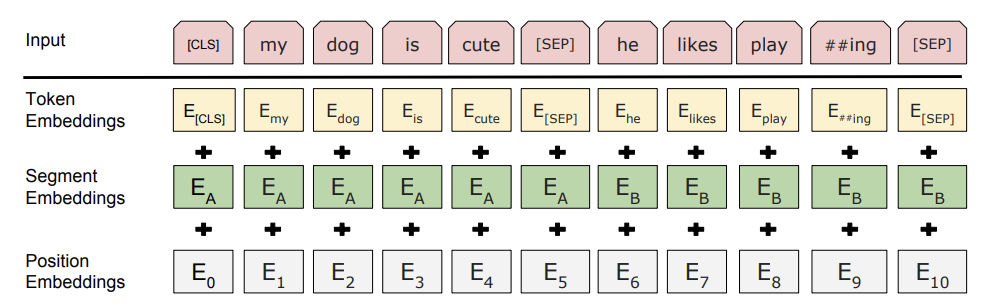
\includegraphics[width=0.9\textwidth]{assets/pics/BERT/bert_representation.png}
\caption{Representasi \textit{input} BERT yang terdiri dari \textit{token}, \textit{segment}, dan \textit{position embedding} \parencite{devlin2018bert}}
\label{fig:bert_input}
\end{figure}

Selain token hasil tokenisasi, BERT menambahkan token khusus \texttt{[CLS]} pada awal urutan \textit{input}. Representasi token tersebut kemudian diproses bersama token lainnya melalui seluruh lapisan \textit{Transformer Encoder} sehingga dapat digunakan sebagai representasi agregat dari urutan teks. Gabungan seluruh vektor $\mathbf{E}_i$ menjadi masukan awal bagi tumpukan \textit{Transformer Encoder}:

\begin{equation}
\mathbf{H}^{(0)} = \mathbf{E} = [\mathbf{E}_{[\text{CLS}]}, \mathbf{E}_1, \mathbf{E}_2, \ldots, \mathbf{E}_n].
\end{equation}

%-------------------------------------------------------------------------%
\subsection{Arsitektur BERT}
\label{subsec:bert_arch}
%-------------------------------------------------------------------------%

Representasi awal $\mathbf{H}^{(0)}$ dilewatkan melalui $L$ lapisan \textit{Transformer Encoder} yang memiliki struktur identik (Gambar~\ref{fig:bert_architecture}). Pada setiap lapisan, representasi tersebut diperbarui melalui mekanisme \textit{self-attention} dan \textit{Position-wise Feed-Forward Network} (FFN), sehingga diperoleh urutan representasi:

\begin{equation}
\mathbf{H}^{(0)} \rightarrow \mathbf{H}^{(1)} \rightarrow \cdots \rightarrow \mathbf{H}^{(L)}.
\end{equation}

\begin{figure}[H]
\centering
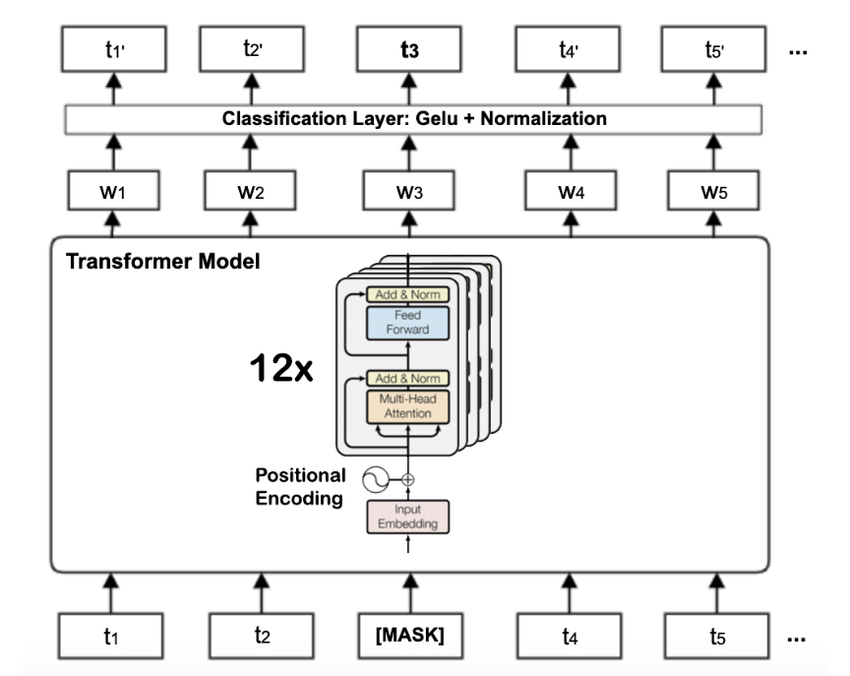
\includegraphics[width=0.6\textwidth]{assets/pics/BERT/Encoder_Stack_BERT.png}
\caption{Tumpukan $L$ lapisan \textit{Transformer Encoder} pada BERT \parencite{devlin2018bert}}
\label{fig:bert_architecture}
\end{figure}

Setiap lapisan \textit{Transformer Encoder} terdiri atas dua sub-lapisan utama, yaitu \textit{Multi-Head Self-Attention} dan \textit{Position-wise Feed-Forward Network} (FFN). Kedua sub-lapisan tersebut dilengkapi dengan koneksi residual dan normalisasi lapisan melalui mekanisme \textit{Add \& Norm} (Gambar~\ref{fig:bert_encoder_layer}). Secara matematis, keluaran dari setiap lapisan dihitung sebagai:

\begin{align}
\mathbf{H}^{(\ell)}_{\text{attn}} &= \text{LayerNorm}\!\left(\mathbf{H}^{(\ell-1)} + \text{MultiHeadAttention}(\mathbf{H}^{(\ell-1)})\right), \\
\mathbf{H}^{(\ell)} &= \text{LayerNorm}\!\left( \mathbf{H}^{(\ell)}_{\text{attn}} + \text{FFN}(\mathbf{H}^{(\ell)}_{\text{attn}})\right).
\end{align}

\begin{figure}[H]
\centering
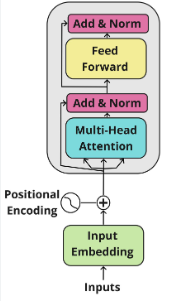
\includegraphics[width=0.3\textwidth]{assets/pics/BERT/Transfomer_Encoder_Layer.png}
\caption{Struktur satu lapisan \textit{Transformer Encoder} \parencite{devlin2018bert}}
\label{fig:bert_encoder_layer}
\end{figure}

Jumlah lapisan $L$, dimensi \textit{hidden state} $d$, dan jumlah \textit{attention head} $h$ bergantung pada varian BERT yang digunakan. Konfigurasi parameter BERT pada penelitian ini dijelaskan pada Bab Metodologi.

%-------------------------------------------------------------------------%
\subsection{Mekanisme \textit{Self-Attention}}
\label{subsec:bert_attention}
%-------------------------------------------------------------------------%

Mekanisme \textit{Multi-Head Self-Attention} memungkinkan setiap token memperhatikan token lain dalam suatu urutan berdasarkan tingkat relevansinya. \textit{Input} $\mathbf{H}^{(\ell-1)} \in \mathbb{R}^{n \times d}$ diproyeksikan menjadi tiga representasi, yaitu \textit{query} ($\mathbf{Q}$), \textit{key} ($\mathbf{K}$), dan \textit{value} ($\mathbf{V}$), melalui matriks bobot yang dipelajari selama proses pelatihan:

\begin{align}
\mathbf{Q} &= \mathbf{H}^{(\ell-1)}\mathbf{W}_Q \in \mathbb{R}^{n \times d_k}, \\
\mathbf{K} &= \mathbf{H}^{(\ell-1)}\mathbf{W}_K \in \mathbb{R}^{n \times d_k}, \\
\mathbf{V} &= \mathbf{H}^{(\ell-1)}\mathbf{W}_V \in \mathbb{R}^{n \times d_v}.
\end{align}

Dalam mekanisme ini, \textit{query} digunakan untuk menghitung tingkat kesesuaian dengan token lain, \textit{key} berfungsi sebagai representasi pembanding dalam perhitungan relevansi, sedangkan \textit{value} menyediakan informasi yang akan dikombinasikan berdasarkan bobot \textit{attention}. Skor relevansi antar-token diperoleh melalui perkalian $\mathbf{Q}\mathbf{K}^\top$, kemudian diskalakan dengan $\sqrt{d_k}$ dan dinormalisasi menggunakan fungsi \textit{softmax} untuk menghasilkan bobot \textit{attention}:

\begin{equation}
\text{Attention}(\mathbf{Q}, \mathbf{K}, \mathbf{V}) = \text{softmax}\!\left(\frac{\mathbf{Q}\mathbf{K}^\top}{\sqrt{d_k}} \right)\mathbf{V}.
\label{eq:attention}
\end{equation}

Untuk menangkap hubungan antar-token dari beberapa ruang representasi yang berbeda, BERT menggunakan beberapa \textit{attention head} yang bekerja secara paralel sebanyak $h$ buah (\textit{Multi-Head Attention}, Gambar~\ref{fig:multihead_attention}). Hasil dari setiap \textit{head} kemudian digabungkan dan diproyeksikan kembali ke dimensi semula:

\begin{equation}
\text{MultiHead}(\mathbf{Q}, \mathbf{K}, \mathbf{V}) = \text{Concat}(\text{head}_1, \ldots, \text{head}_h)\,\mathbf{W}_O.
\end{equation}

\noindent dengan $\text{head}_i = \text{Attention}(\mathbf{Q}\mathbf{W}_Q^i,\, \mathbf{K}\mathbf{W}_K^i,\, \mathbf{V}\mathbf{W}_V^i)$. Pada BERT-Base, jumlah \textit{attention head} yang digunakan adalah $h=12$ dengan dimensi masing-masing $\mathbf{Q}$ dan $\mathbf{K}$ sebesar $d_k=64$, serta $\mathbf{V}$ sebesar $d_v=64$.

\begin{figure}[H]
\centering
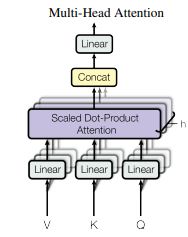
\includegraphics[width=0.3\textwidth]{assets/pics/BERT/transformer_attention.png}
\caption{Mekanisme \textit{Scaled Dot-Product Attention} pada \textit{Multi-Head Attention} \parencite{vaswani2017attention}}
\label{fig:multihead_attention}
\end{figure}

%-------------------------------------------------------------------------%
\subsection{Ekstraksi Fitur dari Token \texttt{[CLS]}}
\label{subsec:bert_feature}
%-------------------------------------------------------------------------%

Setelah melewati $L$ lapisan \textit{Transformer Encoder}, diperoleh \textit{hidden state} akhir $\mathbf{H}^{(L)}$ yang berisi representasi kontekstual dari seluruh token pada urutan input. Pada penelitian ini, representasi token \texttt{[CLS]} pada lapisan terakhir digunakan sebagai vektor fitur untuk setiap dokumen:

\begin{equation}
\mathbf{f} = \mathbf{H}^{(L)}_{[\text{CLS}]} \in \mathbb{R}^{d}.
\end{equation}

\noindent dengan $d$ merupakan dimensi \textit{hidden state} yang bergantung pada varian BERT yang digunakan. Token \texttt{[CLS]} dipilih karena representasinya telah diproses bersama seluruh token lainnya melalui mekanisme \textit{self-attention}, sehingga dapat digunakan sebagai representasi agregat dari suatu urutan teks. Karena parameter BERT dibekukan (\textit{frozen}) selama proses pelatihan, vektor fitur $\mathbf{f}$ diperoleh melalui proses \textit{forward pass} tanpa adanya pembaruan bobot. Selanjutnya, vektor tersebut digunakan sebagai masukan bagi \textit{autoencoder} untuk tahap reduksi dimensi.

%-------------------------------------------------------------------------%
\section{Multi-Task Learning}
%-------------------------------------------------------------------------%

\textit{Multi-Task Learning} (MTL) merupakan pendekatan dalam
\textit{machine learning} yang bertujuan meningkatkan kemampuan
generalisasi model dengan memanfaatkan informasi dari beberapa tugas yang
saling berkaitan secara bersamaan \parencite{caruana1997multitask}. Ketika
dua tugas memiliki keterkaitan, informasi pembelajaran dari satu tugas
dapat membantu tugas lainnya karena keduanya berbagi pola atau struktur
yang sama dalam data.

Konsep kunci yang mendasari MTL adalah \textit{inductive transfer}, yaitu
kemampuan model untuk memindahkan pengetahuan yang dipelajari dari satu
tugas ke tugas lainnya. \parencite{caruana1997multitask} menjelaskan bahwa
MTL mencapai hal ini dengan cara mempelajari beberapa tugas secara paralel
menggunakan representasi bersama. Tugas-tugas lain berfungsi sebagai
\textit{inductive bias}, yaitu mekanisme yang mengarahkan model agar
mempelajari hipotesis yang dapat menjelaskan lebih dari satu tugas
sekaligus \parencite{ruder2017overview}.

Pada penelitian ini, MTL digunakan untuk mempelajari analisis sentimen dan
pendeteksian topik secara bersamaan. Kedua tugas ini memiliki keterkaitan
yang kuat karena sama-sama bergantung pada pemahaman semantis teks ulasan,
sehingga representasi yang berguna untuk mendeteksi topik juga cenderung
berguna untuk mengklasifikasikan sentimen.

%-------------------------------------------------------------------------%
\subsection{Formulasi MTL}
%-------------------------------------------------------------------------%

Misalkan terdapat $T$ tugas yang dipelajari secara bersamaan. Untuk setiap
tugas $t \in \{1, 2, \ldots, T\}$, terdapat dataset
$\mathcal{D}_t = \{(\mathbf{x}_i^{(t)}, y_i^{(t)})\}_{i=1}^{n_t}$ dan
fungsi \textit{loss} $\mathcal{L}_t$ yang mengukur kesalahan prediksi pada
tugas ke-$t$. Karena MTL mempelajari beberapa tugas secara bersamaan,
proses optimasi dilakukan dengan menggabungkan kontribusi seluruh fungsi
\textit{loss} ke dalam satu fungsi objektif:

\begin{equation}
    \mathcal{L}_{\text{MTL}} = \sum_{t=1}^{T} \alpha_t
    \mathcal{L}_t(\theta_t, \theta_{\text{shared}}).
    \label{eq:mtl_objective}
\end{equation}

\noindent dengan $\alpha_t$ adalah skalar bobot yang mengontrol seberapa besar
kontribusi tugas ke-$t$ terhadap total \textit{loss}, $\theta_t$ adalah
parameter yang spesifik untuk tugas ke-$t$, dan $\theta_{\text{shared}}$
adalah parameter yang dibagikan bersama oleh semua tugas. Parameter
optimal diperoleh dengan meminimalkan
persamaan~\eqref{eq:mtl_objective} secara bersama-sama:

\begin{equation}
    \theta_{\text{shared}}^*, \{\theta_t^*\}_{t=1}^{T} =
    \argmin_{\theta_{\text{shared}}, \{\theta_t\}}
    \mathcal{L}_{\text{MTL}}.
    \label{eq:mtl_optimization}
\end{equation}

Pada penelitian ini, fungsi \textit{loss} total terdiri dari dua
komponen. Komponen pertama adalah \textit{clustering loss} berbasis
\textit{Kullback-Leibler Divergence} (KLD), yang mengoptimalkan jarak
antara distribusi penugasan klaster $Q$ dan distribusi target $P$.
Komponen kedua adalah \textit{sentiment loss} berbasis
\textit{categorical cross-entropy} untuk klasifikasi sentimen. Keduanya
digabungkan sebagai berikut:

\begin{equation}
    \mathcal{L}_{\text{MTL}} = \alpha_1 \cdot \mathcal{L}_{\text{cluster}}
    + \alpha_2 \cdot \mathcal{L}_{\text{sentiment}}.
    \label{eq:loss_total}
\end{equation}

\noindent dengan $\alpha_1$ dan $\alpha_2$ adalah skalar hiperparameter yang
mengontrol bobot masing-masing komponen. \textit{Clustering loss}
diformulasikan sebagai KLD antara distribusi target $P$ dan distribusi
penugasan $Q$:

\begin{equation}
    \mathcal{L}_{\text{cluster}} = D_{KL}(P \| Q)
    = \sum_{i} \sum_{j} p_{ij} \log \frac{p_{ij}}{q_{ij}}.
    \label{eq:kld_loss}
\end{equation}

\noindent dengan $q_{ij}$ adalah probabilitas sampel ke-$i$ termasuk ke klaster
ke-$j$, dan $p_{ij}$ adalah distribusi target yang diturunkan dari $Q$
sebagai berikut:

\begin{equation}
    p_{ij} = \frac{q_{ij}^2 / \sum_i q_{ij}}{\sum_{j'} q_{ij'}^2 /
    \sum_i q_{ij'}}.
    \label{eq:target_distribution}
\end{equation}

Pembagian dengan $\sum_i q_{ij}$ menormalisasi frekuensi klaster agar
klaster yang besar tidak mendominasi, sedangkan operasi kuadrat pada
$q_{ij}$ membuat distribusi keanggotaan lebih terkonsentrasi pada satu
klaster.

%-------------------------------------------------------------------------%
\subsection{\textit{Hard Parameter Sharing}}
%-------------------------------------------------------------------------%

\textit{Hard parameter sharing} merupakan pendekatan MTL yang paling umum
digunakan dalam \textit{deep learning} \parencite{ruder2017overview}. Pada
pendekatan ini, lapisan tersembunyi bersifat \textit{shared} antar semua
tugas, sementara setiap tugas memiliki lapisan \textit{output} tersendiri.
Secara formal, untuk input $\mathbf{x}$, proses komputasinya adalah:

\begin{align}
    \mathbf{h}_{\text{shared}} &= f_{\text{shared}}(\mathbf{x};\,
        \theta_{\text{shared}}), \label{eq:hard_shared} \\
    \hat{y}_t &= f_t(\mathbf{h}_{\text{shared}};\, \theta_t),
        \quad t = 1, \ldots, T. \label{eq:hard_task}
\end{align}

\noindent dengan $f_{\text{shared}}$ adalah jaringan bersama yang menghasilkan
vektor representasi $\mathbf{h}_{\text{shared}}$, dan $f_t$ adalah
jaringan spesifik tugas ke-$t$. \parencite{baxter2000model} menunjukkan
secara teoritis bahwa mekanisme ini mengurangi risiko \textit{overfitting}
karena gradien dari semua tugas mengalir ke lapisan bersama selama
\textit{backpropagation}. Arsitektur \textit{hard parameter sharing}
diilustrasikan pada Gambar~\ref{fig:hard_sharing}.

\begin{figure}[H]
\centering
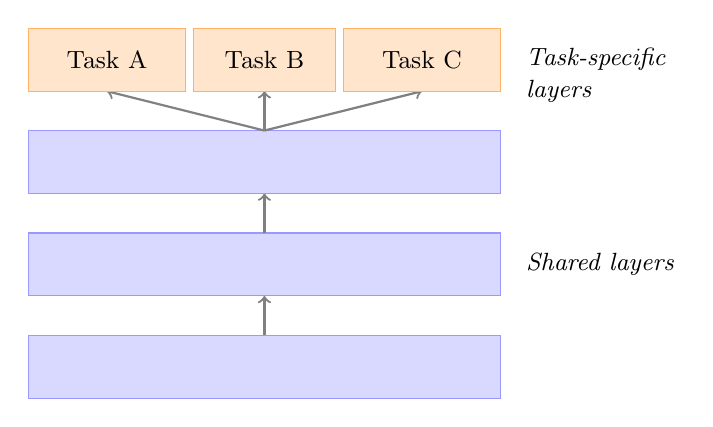
\begin{tikzpicture}[
    arr/.style={->, thick, gray}
]

    % Shared layer 1
    \fill[blue!15] (-3, 0) rectangle (3, 0.8);
    \draw[blue!40] (-3, 0) rectangle (3, 0.8);

    % Arrow between shared layer 1 and 2
    \draw[arr] (0, 0.8) -- (0, 1.3);

    % Shared layer 2
    \fill[blue!15] (-3, 1.3) rectangle (3, 2.1);
    \draw[blue!40] (-3, 1.3) rectangle (3, 2.1);

    % Arrow between shared layer 2 and 3
    \draw[arr] (0, 2.1) -- (0, 2.6);

    % Shared layer 3
    \fill[blue!15] (-3, 2.6) rectangle (3, 3.4);
    \draw[blue!40] (-3, 2.6) rectangle (3, 3.4);

    \node[right] at (3.2, 1.7) {\small \textit{Shared layers}};

    % Arrows from shared layer 3 to each task (diagonal)
    \draw[arr] (0, 3.4) -- (-2, 3.9);
    \draw[arr] (0, 3.4) -- (0,  3.9);
    \draw[arr] (0, 3.4) -- (2,  3.9);

    % Task-specific: 3 kotak terpisah
    \fill[orange!20] (-3,   3.9) rectangle (-1,   4.7);
    \fill[orange!20] (-0.9, 3.9) rectangle (0.9,  4.7);
    \fill[orange!20] (1,    3.9) rectangle (3,    4.7);
    \draw[orange!60] (-3,   3.9) rectangle (-1,   4.7);
    \draw[orange!60] (-0.9, 3.9) rectangle (0.9,  4.7);
    \draw[orange!60] (1,    3.9) rectangle (3,    4.7);

    \node at (-2,  4.3) {\small Task A};
    \node at (0,   4.3) {\small Task B};
    \node at (2,   4.3) {\small Task C};
    \node[right] at (3.2, 4.3) {\small \textit{Task-specific}};
    \node[right] at (3.2, 3.9) {\small \textit{layers}};

\end{tikzpicture}
\caption{Ilustrasi arsitektur \textit{hard parameter sharing} dalam
\textit{Multi-Task Learning} (\cite{ruder2017overview}, telah diolah
kembali)}
\label{fig:hard_sharing}
\end{figure}

Pada penelitian ini, pendekatan \textit{hard parameter sharing} diterapkan
dengan menjadikan \textit{autoencoder} sebagai jaringan bersama.
Representasi laten $\mathbf{z}$ yang dihasilkan oleh \textit{encoder}
digunakan secara bersamaan oleh dua \textit{head}: satu untuk pendeteksian
topik melalui \textit{clustering layer}, dan satu lagi untuk klasifikasi
sentimen melalui \textit{sentiment classifier}.

%-------------------------------------------------------------------------%
\subsection{\textit{Soft Parameter Sharing}}
%-------------------------------------------------------------------------%

\textit{Soft parameter sharing} mengambil pendekatan yang berbeda. Setiap
tugas memiliki model tersendiri dengan parameter masing-masing, namun
parameter antar model diatur agar tidak terlalu jauh berbeda melalui
regularisasi \parencite{ruder2017overview}. Salah satu cara yang umum
digunakan adalah menambahkan penalti $\ell_2$ terhadap perbedaan parameter
antar tugas:

\begin{equation}
    \mathcal{L}_{\text{soft}} = \sum_{t=1}^{T} \mathcal{L}_t(\theta_t)
    + \lambda \sum_{t=1}^{T} \sum_{t'=t+1}^{T}
    \|\theta_t - \theta_{t'}\|_2^2.
    \label{eq:soft_l2_reg}
\end{equation}

\noindent dengan $\lambda$ adalah skalar koefisien regularisasi yang mengontrol
seberapa mirip parameter antar tugas harus dijaga, dan
$\|\theta_t - \theta_{t'}\|_2^2$ mengukur seberapa jauh kedua set
parameter berbeda. Arsitektur \textit{soft parameter sharing}
diilustrasikan pada Gambar~\ref{fig:soft_sharing}.

\begin{figure}[H]
\centering
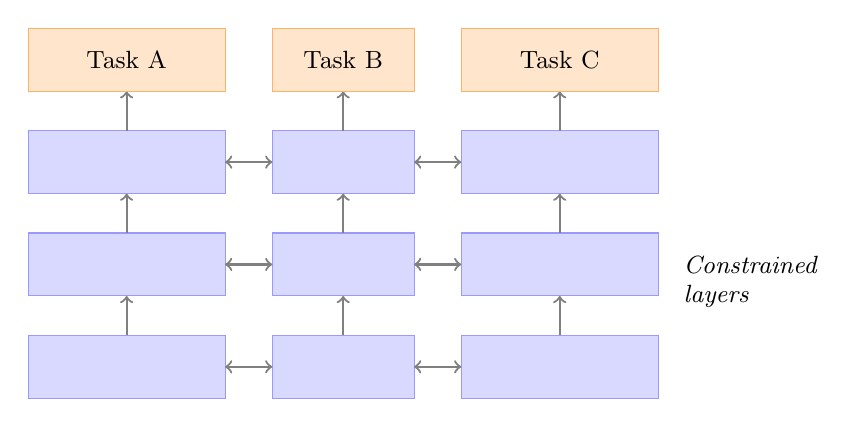
\begin{tikzpicture}[
    arr/.style={->, thick, gray},
    darr/.style={<->, thick, gray}
]
    % Constrained layer 1 (bottom)
    \fill[blue!15] (-4, 0) rectangle (-1.5, 0.8);
    \draw[blue!40] (-4, 0) rectangle (-1.5, 0.8);
    \fill[blue!15] (-0.9, 0) rectangle (0.9, 0.8);
    \draw[blue!40] (-0.9, 0) rectangle (0.9, 0.8);
    \fill[blue!15] (1.5, 0) rectangle (4, 0.8);
    \draw[blue!40] (1.5, 0) rectangle (4, 0.8);

    % Horizontal arrows layer 1
    \draw[darr] (-1.5, 0.4) -- (-0.9, 0.4);
    \draw[darr] (0.9, 0.4) -- (1.5, 0.4);

    % Arrows up layer 1 to 2
    \draw[arr] (-2.75, 0.8) -- (-2.75, 1.3);
    \draw[arr] (0, 0.8) -- (0, 1.3);
    \draw[arr] (2.75, 0.8) -- (2.75, 1.3);

    % Constrained layer 2 (middle)
    \fill[blue!15] (-4, 1.3) rectangle (-1.5, 2.1);
    \draw[blue!40] (-4, 1.3) rectangle (-1.5, 2.1);
    \fill[blue!15] (-0.9, 1.3) rectangle (0.9, 2.1);
    \draw[blue!40] (-0.9, 1.3) rectangle (0.9, 2.1);
    \fill[blue!15] (1.5, 1.3) rectangle (4, 2.1);
    \draw[blue!40] (1.5, 1.3) rectangle (4, 2.1);

    % Horizontal arrows layer 2
    \draw[darr] (-1.5, 1.7) -- (-0.9, 1.7);
    \draw[darr] (0.9, 1.7) -- (1.5, 1.7);

    % Arrows up layer 2 to 3
    \draw[arr] (-2.75, 2.1) -- (-2.75, 2.6);
    \draw[arr] (0, 2.1) -- (0, 2.6);
    \draw[arr] (2.75, 2.1) -- (2.75, 2.6);

    % Constrained layer 3 (top constrained)
    \fill[blue!15] (-4, 2.6) rectangle (-1.5, 3.4);
    \draw[blue!40] (-4, 2.6) rectangle (-1.5, 3.4);
    \fill[blue!15] (-0.9, 2.6) rectangle (0.9, 3.4);
    \draw[blue!40] (-0.9, 2.6) rectangle (0.9, 3.4);
    \fill[blue!15] (1.5, 2.6) rectangle (4, 3.4);
    \draw[blue!40] (1.5, 2.6) rectangle (4, 3.4);

    % Horizontal arrows layer 3
    \draw[darr] (-1.5, 3.0) -- (-0.9, 3.0);
    \draw[darr] (0.9, 3.0) -- (1.5, 3.0);

    \node[right] at (4.2, 1.7) {\small \textit{Constrained}};
    \node[right] at (4.2, 1.3) {\small \textit{layers}};

    % Arrows up to task boxes
    \draw[arr] (-2.75, 3.4) -- (-2.75, 3.9);
    \draw[arr] (0, 3.4) -- (0, 3.9);
    \draw[arr] (2.75, 3.4) -- (2.75, 3.9);

    % Task boxes
    \fill[orange!20] (-4, 3.9) rectangle (-1.5, 4.7);
    \draw[orange!60] (-4, 3.9) rectangle (-1.5, 4.7);
    \fill[orange!20] (-0.9, 3.9) rectangle (0.9, 4.7);
    \draw[orange!60] (-0.9, 3.9) rectangle (0.9, 4.7);
    \fill[orange!20] (1.5, 3.9) rectangle (4, 4.7);
    \draw[orange!60] (1.5, 3.9) rectangle (4, 4.7);

    \node at (-2.75, 4.3) {\small Task A};
    \node at (0, 4.3) {\small Task B};
    \node at (2.75, 4.3) {\small Task C};

\end{tikzpicture}
\caption{Ilustrasi arsitektur \textit{soft parameter sharing}
(\cite{ruder2017overview}, telah diolah kembali)}
\label{fig:soft_sharing}
\end{figure}

Perbedaan mendasar antara keduanya terletak pada bagaimana pengetahuan
dibagikan. Pada \textit{hard parameter sharing}, bobot benar-benar identik
sehingga semua tugas menggunakan representasi yang sama persis. Pada
\textit{soft parameter sharing}, setiap tugas tetap memiliki ruang belajar
sendiri namun didorong untuk tidak terlalu menyimpang, sehingga lebih
fleksibel namun membutuhkan lebih banyak parameter dan pengaturan
$\lambda$ yang tepat.

%-------------------------------------------------------------------------%
\section{\textit{Clustering}}
%-------------------------------------------------------------------------%

\textit{Clustering} merupakan teknik \textit{unsupervised learning} yang
mengelompokkan data berdasarkan kemiripan tanpa memerlukan label
\parencite{bezdek1984}. Berdasarkan cara pengelompokannya, terdapat dua
pendekatan utama. \textit{Hard clustering} membatasi setiap titik data ke
satu klaster, sedangkan \textit{soft clustering} memungkinkan satu titik
data masuk ke beberapa klaster sekaligus.

Metode \textit{clustering} dapat diklasifikasikan ke dalam beberapa
pendekatan, di antaranya \textit{centroid-based}, \textit{distribution-based},
\textit{connectivity-based}, dan \textit{density-based}. Penelitian ini
menggunakan pendekatan \textit{centroid-based clustering}, yaitu metode yang
memisahkan data berdasarkan jarak setiap titik data terhadap pusat klaster
(\textit{centroid}) \parencite{yusdiansyah2019}. Untuk mengukur jarak
tersebut digunakan jarak Euclidean:

\begin{equation}
    \|\mathbf{p} - \mathbf{q}\| =
    \sqrt{\sum_{d=1}^{D}(p_d - q_d)^2}.
    \label{eq:euclidean_distance}
\end{equation}

\noindent dengan $\mathbf{p} = (p_1, \ldots, p_D)$ dan
$\mathbf{q} = (q_1, \ldots, q_D)$ adalah dua vektor dalam ruang
berdimensi $D$.

Penelitian ini menggunakan \textit{Deep Embedded Clustering} (DEC)
\parencite{xie2016unsupervised} sebagai metode pendeteksian topik, yang
mempelajari representasi laten dan melakukan \textit{clustering} secara
bersamaan. DEC menerapkan \textit{soft clustering} melalui distribusi
probabilitas penugasan klaster, sehingga setiap ulasan dapat terhubung ke
lebih dari satu topik. Sebagai inisialisasi, DEC menggunakan K-Means untuk
menentukan pusat klaster awal di ruang \textit{embedding}.

%-------------------------------------------------------------------------%
\subsection{K-Means \textit{Clustering}}
%-------------------------------------------------------------------------%

K-Means merupakan algoritma \textit{centroid-based clustering} yang
mengelompokkan data dengan meminimalkan total jarak antara setiap titik
data dan pusat klasternya, dan termasuk ke dalam kategori \textit{hard
clustering} \parencite{macqueen1967some}.

Secara formal, misalkan terdapat himpunan data $X = \{\mathbf{x}_1,
\mathbf{x}_2, \ldots, \mathbf{x}_N\}$ dengan $\mathbf{x}_n \in
\mathbb{R}^D$ dan jumlah klaster yang diinginkan adalah $K$. K-Means
meminimalkan fungsi objektif berikut:

\begin{equation}
    J = \sum_{n=1}^{N} \sum_{k=1}^{K} r_{nk}
    \|\mathbf{x}_n - \boldsymbol{\mu}_k\|^2.
    \label{eq:kmeans_objective}
\end{equation}

\noindent dengan $\boldsymbol{\mu}_k$ adalah vektor \textit{centroid} klaster
ke-$k$, dan $r_{nk}$ adalah skalar variabel indikator biner yang bernilai
1 jika titik data $\mathbf{x}_n$ termasuk klaster ke-$k$ dan 0 jika
tidak. Nilai $J$ mengukur total kuadrat jarak seluruh titik data ke pusat
klasternya masing-masing.

Proses optimasi dilakukan secara iteratif melalui dua tahap yang
bergantian. Pada tahap pertama (\textit{assignment step}), setiap titik
data dialokasikan ke klaster dengan \textit{centroid} terdekat:

\begin{equation}
    r_{nk} = \begin{cases}
        1, & k = \arg\min_j \|\mathbf{x}_n - \boldsymbol{\mu}_j\|^2 \\
        0, & \text{yang lainnya.}
    \end{cases}
    \label{eq:assignment_step}
\end{equation}

\noindent dengan $\arg\min_j \|\mathbf{x}_n - \boldsymbol{\mu}_j\|^2$
menyatakan indeks $j$ yang meminimalkan nilai
$\|\mathbf{x}_n - \boldsymbol{\mu}_j\|^2$, yaitu indeks \textit{centroid}
terdekat terhadap titik data $\mathbf{x}_n$. Notasi $\arg\max$ yang
digunakan pada bagian-bagian selanjutnya memiliki pengertian yang serupa,
yaitu mengembalikan indeks yang memaksimalkan suatu fungsi.

Pada tahap kedua (\textit{update step}), \textit{centroid} setiap klaster
diperbarui menjadi rata-rata dari seluruh titik yang menjadi anggotanya:

\begin{equation}
    \boldsymbol{\mu}_k = \frac{\sum_{n=1}^{N} r_{nk}\,
    \mathbf{x}_n}{\sum_{n=1}^{N} r_{nk}}.
    \label{eq:centroid_update}
\end{equation}

Pembilang adalah jumlah posisi seluruh anggota klaster ke-$k$, sedangkan
penyebut adalah jumlah anggotanya. Dua tahap ini diulang sampai nilai $J$
tidak berubah signifikan atau jumlah iterasi mencapai batas maksimum.
Algoritma lengkapnya dapat dilihat pada Tabel~\ref{tab:kmeans_algorithm}.

\begin{table}[H]
\centering
\footnotesize
\setlength{\tabcolsep}{4pt}
\renewcommand{\arraystretch}{0.95}
\caption{Algoritma K-Means \textit{Clustering}}
\label{tab:kmeans_algorithm}
\resizebox{\textwidth}{!}{
\begin{tabular}{p{12cm}}
\toprule
\textbf{Algoritma K-Means \textit{Clustering}} \\
\midrule
\textbf{INPUT:} Himpunan data $\{\mathbf{x}_i\}_{i=1}^N$, banyak klaster
$K$, batas toleransi $\epsilon$, dan maksimal iterasi $\text{maxiter}$ \\
\midrule
1. Inisialisasi secara acak himpunan \textit{centroid}
   $\{\boldsymbol{\mu}_j\}_{j=1}^K$ \\
2. Tetapkan $\text{iter} = 0$ \\
3. \textbf{REPEAT} \\
4. \quad Tetapkan $\text{iter} = \text{iter} + 1$ \\
5. \quad \textit{Assignment step:} Cari nilai
$r_{nk} =
\begin{cases}
1, & k = \arg\min_j \|\mathbf{x}_n - \boldsymbol{\mu}_j\|^2 \\
0, & \text{yang lainnya}
\end{cases}$ \\
6. \quad \textit{Update step:} Cari nilai
$\boldsymbol{\mu}_k =
\frac{\sum_{n=1}^N r_{nk} \mathbf{x}_n}{\sum_{n=1}^N r_{nk}}$ \\
7. \quad Hitung
$J = \sum_{n=1}^N \sum_{k=1}^K r_{nk}
\|\mathbf{x}_n - \boldsymbol{\mu}_k\|^2$ \\
8. \textbf{UNTIL} $J < \epsilon$ \textbf{OR}
   $\text{iter} > \text{maxiter}$ \\
9. Untuk setiap $n = 1, 2, \ldots, N$, tetapkan nilai
   $u_n = \arg\max_k (r_{nk})$, dengan $k = 1, 2, \ldots, K$ \\
10. Bentuk $\{C_1, C_2, \ldots, C_K\}$, dengan $C_k$ merupakan himpunan
    anggota data $\mathbf{x}_i$ di mana $u_i = k$ \\
11. \textbf{STOP} \\
\midrule
\textbf{OUTPUT:} Nilai keanggotaan $\{u_n\}_{n=1}^N$ dan himpunan klaster
$\{C_k\}_{k=1}^K$ \\
\bottomrule
\end{tabular}
}
\end{table}

%-------------------------------------------------------------------------%
\section{Interpretabilitas Model \textit{Deep Learning}}
%-------------------------------------------------------------------------%

Interpretabilitas model \textit{deep learning} merujuk pada kemampuan
untuk memahami dan menjelaskan keputusan yang dihasilkan oleh model yang
bersifat \textit{black-box} \parencite{sundararajan2017axiomatic}. Dalam
konteks pemrosesan bahasa alami, interpretabilitas penting karena model
perlu mampu menjelaskan mengapa suatu teks diklasifikasikan ke dalam
kategori tertentu, terutama pada aplikasi analisis sentimen dan
pengelompokan topik.

Secara umum, metode interpretabilitas dapat dikategorikan menjadi dua
kelompok \parencite{li2016visualizing}. Kelompok pertama adalah metode
\textit{intrinsic}, yaitu model yang secara bawaan dapat diinterpretasi
seperti pohon keputusan dan regresi linier. Kelompok kedua adalah metode
\textit{post-hoc}, yaitu metode yang diterapkan setelah model dilatih
untuk menganalisis perilaku model yang kompleks tanpa mengubah
arsitekturnya.

Dalam penelitian ini, metode \textit{post-hoc} digunakan untuk menganalisis
kontribusi setiap token terhadap prediksi sentimen model, yaitu
\textit{occlusion-based token attribution} dan \textit{Integrated
Gradients}.

%-------------------------------------------------------------------------%
\subsection{\textit{Occlusion-based Token Attribution}}
%-------------------------------------------------------------------------%

\textit{Occlusion-based token attribution} merupakan salah satu metode
\textit{post-hoc} yang banyak digunakan untuk menginterpretasi model
berbasis teks \parencite{zeiler2014visualizing, li2016visualizing}. Metode
ini mengukur pentingnya suatu token dengan cara menggantinya dan mengamati
perubahan prediksi model.

Pada model berbasis \textit{transformer} seperti BERT, oklusi dilakukan
dengan mengganti token target menggunakan token khusus \texttt{[MASK]},
sehingga model tetap menerima input dengan panjang yang sama. Pendekatan
ini dikenal sebagai \textit{leave-one-out attribution}.

Secara formal, diberikan teks input $\mathbf{x} = (x_1, x_2, \ldots,
x_T)$ yang terdiri dari $T$ token, representasi kontekstual diperoleh
melalui BERT sebagai:

\begin{equation}
    \mathbf{h} = \text{BERT}(\mathbf{x}) \in \mathbb{R}^d.
    \label{eq:bert_cls}
\end{equation}

\noindent dengan $\mathbf{h}$ merupakan vektor representasi \texttt{[CLS]} dari
lapisan terakhir BERT. Representasi ini kemudian diteruskan ke lapisan
klasifikasi sentimen untuk menghasilkan distribusi probabilitas:

\begin{equation}
    f(\mathbf{x}) = \text{softmax}(\mathbf{W} \cdot \mathbf{h} + \mathbf{b})
    \in \mathbb{R}^C.
    \label{eq:sentiment_pred}
\end{equation}

\noindent dengan $C$ adalah jumlah kelas sentimen, $\mathbf{W}$ adalah matriks
bobot dan $\mathbf{b}$ adalah vektor bias lapisan klasifikasi. Skor
atribusi token $x_i$ terhadap kelas sentimen $c$ didefinisikan sebagai
selisih probabilitas prediksi sebelum dan sesudah oklusi:

\begin{equation}
    \text{Attr}(x_i, c) = f_c(\mathbf{x}) -
    f_c(\mathbf{x}_{\setminus i}).
    \label{eq:occlusion}
\end{equation}

\noindent dengan $f_c(\mathbf{x})$ adalah skalar probabilitas prediksi kelas $c$
pada teks asli, dan $f_c(\mathbf{x}_{\setminus i})$ adalah skalar
probabilitas prediksi setelah token $x_i$ diganti dengan \texttt{[MASK]}.
Nilai positif berarti token $x_i$ mendukung prediksi kelas $c$, nilai
negatif berarti token menekannya, dan nilai mendekati nol berarti token
tidak berpengaruh signifikan.

Dibandingkan dengan metode berbasis gradien, \textit{occlusion-based
attribution} lebih mudah diinterpretasi karena tidak bergantung pada
komputasi turunan yang kompleks. Namun, metode ini memiliki kompleksitas
waktu $\mathcal{O}(T)$ terhadap panjang token sehingga lebih mahal secara
komputasi untuk teks yang panjang \parencite{li2016visualizing}.

%-------------------------------------------------------------------------%
\subsection{\textit{Integrated Gradients}}
%-------------------------------------------------------------------------%

\textit{Integrated Gradients} (IG) merupakan metode atribusi berbasis
gradien yang diusulkan oleh \parencite{sundararajan2017axiomatic}. Berbeda
dengan \textit{occlusion-based attribution} yang bersifat diskrit, IG
menghitung kontribusi setiap dimensi input secara kontinu dengan
mengintegrasikan gradien prediksi model sepanjang jalur lurus dari
\textit{baseline} menuju input asli.

Secara formal, diberikan vektor input $\mathbf{x} \in \mathbb{R}^d$ dan
vektor \textit{baseline} $\mathbf{x'} \in \mathbb{R}^d$ yang umumnya
berupa vektor nol, atribusi IG untuk dimensi ke-$i$ didefinisikan sebagai:

\begin{equation}
    \text{IG}_i(\mathbf{x}) = (x_i - x'_i) \times
    \int_{\alpha=0}^{1}
    \frac{\partial f\big(\mathbf{x'} + \alpha(\mathbf{x} -
    \mathbf{x'})\big)}{\partial x_i} \, d\alpha.
    \label{eq:ig}
\end{equation}

\noindent dengan $\alpha$ adalah skalar parameter yang menunjukkan posisi pada
jalur dari \textit{baseline} menuju input asli, dan
$\frac{\partial f}{\partial x_i}$ adalah skalar gradien prediksi terhadap
dimensi ke-$i$. Dalam praktiknya, integral tersebut diaproksimasi
menggunakan \textit{Riemann sum} dengan $m$ langkah interpolasi:

\begin{equation}
    \text{IG}_i(\mathbf{x}) \approx (x_i - x'_i) \times
    \sum_{k=1}^{m}
    \frac{\partial f\Big(\mathbf{x'} + \frac{k}{m}
    (\mathbf{x} - \mathbf{x'})\Big)}{\partial x_i} \times
    \frac{1}{m}.
    \label{eq:ig_approx}
\end{equation}

Metode IG memenuhi dua karakteristik penting, yaitu \textit{sensitivity}
dan \textit{implementation invariance}
\parencite{sundararajan2017axiomatic}. \textit{Sensitivity} menjamin bahwa
apabila suatu fitur mempengaruhi prediksi model, fitur tersebut akan
mendapatkan atribusi bernilai tidak nol. \textit{Implementation invariance}
menjamin bahwa dua model yang secara fungsional ekuivalen akan menghasilkan
atribusi yang sama meskipun memiliki implementasi internal yang berbeda.